Um novo experimento foi realizado, avaliando HTU e também a recomendação de algoritmos de aprendizado de máquina em outras condições.
Por conveniência, apenas os aspectos mais relevantes do método experimental adotado nas seções anteriores foram considerados.
Todos os experimentos reportados até este ponto no texto foram baseados no mesmo grupo de algoritmos de aprendizado enquanto aprendizes ativos: 5NNw, C4.5w, NB e SVM.

O novo experimento procura verificar o efeito da adoção, como aprendizes ativos, de um grupo de dois algoritmos baseados em comitê, (aprendiz ativo)RFw e (aprendiz ativo)RoF, possivelmente com maior poder preditivo do que o grupo anterior - conforme discutido no Capítulo \ref{metodologia}.
O uso do prefixo \textit{(aprendiz ativo)} visa evitar ambiguidades com a utilização, em experimentos prévios, desses dois algoritmos em outra tarefa completamente distinta.
Eles são agora adotados como aprendizes contidos nas estratégias, com apenas 10 árvores cada; diferentemente do papel de meta-aprendizes que desempenharam nos experimentos anteriores - em que puderam ser utilizadas 500 árvores.

A Figura \ref{plotfim} contém as curvas de ranqueamento geradas com os dois algoritmos pertencentes ao novo grupo e também a faixa de metaPCT, que alterna entre (aprendiz ativo)RFw e (aprendiz ativo)RoF conforme predito pelo sistema de recomendação automática.
As únicas curvas explícitas são da melhor estratégia de cada faixa, de todas as estratégias da faixa metaPCT e de todos os pares contendo HTUeuc ou SGmulti.
% HTUeuc-RoF, Mar-RFw, HTUeuc-metaPCT, Mar-metaPCT, EERent-metaPCT, SGmulti-metaPCT, HTUeuc-RFw, SGmulti-RoF e SGmulti-RFw.
\begin{figure}[]
\centering
	\includestandalone[mode=buildmissing]{fimPlotfig}
	\caption[Curvas de ranqueamento com faixas RFw, RoF e metaPCT.]{Curvas de ranqueamento com faixas RFw, RoF e metaPCT. Medida comparada: $\mu_{\kappa}$.
	\textit{O limite superior de metaDef coincide com a melhor estratégia de RoF, HTUeuc.}\textit{Detalhes na Figura \ref{curvasrankbands}.}}
	\label{plotfim}
\end{figure}

Como pode ser visto, há uma intersecção expressiva entre as faixas correspondentes aos aprendizes base: (aprendiz ativo)RFw e (aprendiz ativo)RoF.
Consequentemente, em geral, houve pouca margem de exploração do período de consultas (tanto na primeira quanto na segunda metade) por parte do meta-aprendiz PCT e da referência metaDef.
De fato, a região hachurada, que corresponde à faixa de metaPCT, se estende praticamente do topo do gráfico até sua base, com exceção das estreitas áreas de RoF e RFw acima à esquerda e direita, respectivamente; e, RFw abaixo.
Essa observação é confirmada quantitativamente pelo desempenho no nível meta,
de acordo com os valores de ALC-$\mu\kappa$ - conforme apresentado na Figura \ref{alcmetarfrof}.
\begin{figure}
\centering
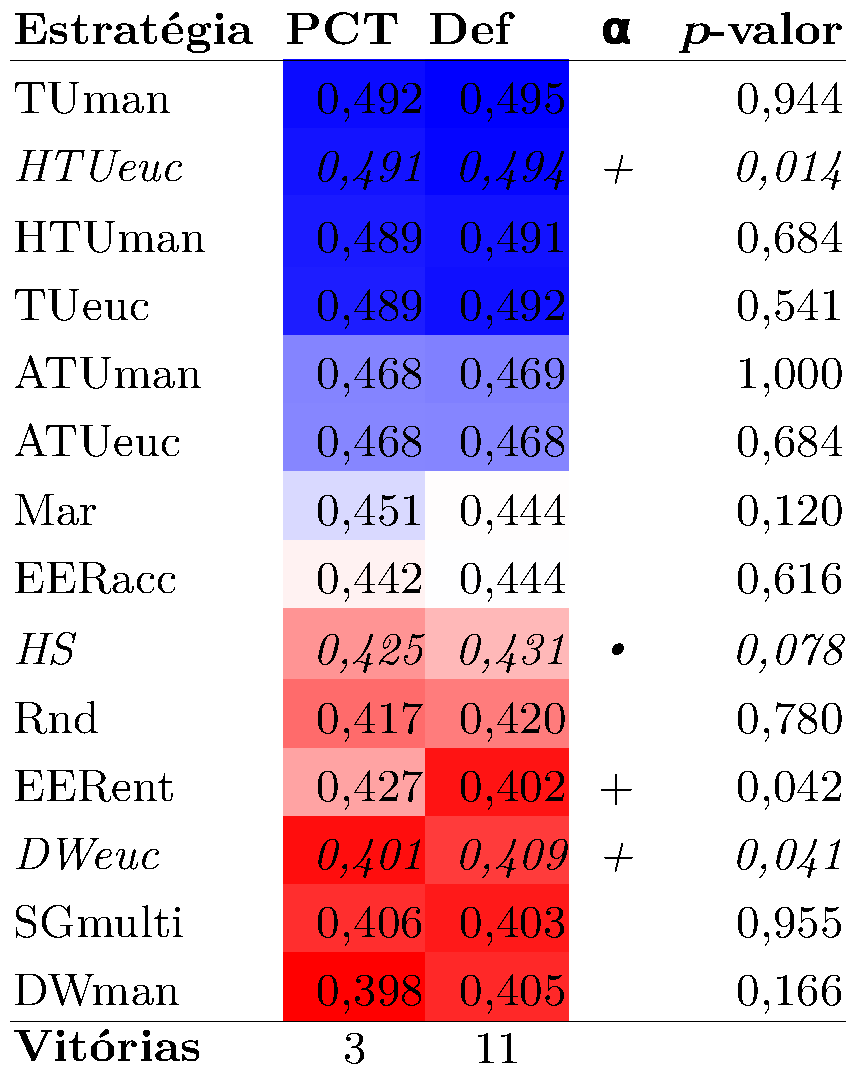
\includegraphics[scale=0.4]{images/metaalcrfrof.pdf}
\caption[Comparação de valores de ALC-$\mu_{\kappa}$ com RFw e RoF como aprendizes.]{Comparação de valores de ALC-$\mu_{\kappa}$ com RFw e RoF como aprendizes.
\textit{Linhas em itálico indicam diferença com significância estatística a favor da referência. Legenda na Tabela \ref{exfried}.}}
\label{alcmetarfrof}
% List(,  Wilcoxon signed rank test with continuity correction, , data:  x and y, V = 32, p-value = 0.6835, alternative hypothesis: true location shift is not equal to 0) <- log)
% List(,  Wilcoxon signed rank test with continuity correction, , data:  x and y, V = 28, p-value = 1, alternative hypothesis: true location shift is not equal to 0) <- log)
% List(,  Wilcoxon signed rank test with continuity correction, , data:  x and y, V = 1190, p-value = 0.6161, alternative hypothesis: true location shift is not equal to 0) <- log)
% List(,  Wilcoxon signed rank test with continuity correction, , data:  x and y, V = 2148, p-value = 4.234e-05, alternative hypothesis: true location shift is not equal to 0) <- log)
% List(,  Wilcoxon signed rank test with continuity correction, , data:  x and y, V = 1286, p-value = 0.07826, alternative hypothesis: true location shift is not equal to 0) <- log)
% List(,  Wilcoxon signed rank test with continuity correction, , data:  x and y, V = 10, p-value = 0.01445, alternative hypothesis: true location shift is not equal to 0) <- log)
% List(,  Wilcoxon signed rank test with continuity correction, , data:  x and y, V = 23, p-value = 0.6835, alternative hypothesis: true location shift is not equal to 0) <- log)
% List(,  Wilcoxon signed rank test with continuity correction, , data:  x and y, V = 792, p-value = 0.0001201, alternative hypothesis: true location shift is not equal to 0) <- log)
% List(,  Wilcoxon signed rank test with continuity correction, , data:  x and y, V = 1681, p-value = 0.7801, alternative hypothesis: true location shift is not equal to 0) <- log)
% List(,  Wilcoxon signed rank test with continuity correction, , data:  x and y, V = 327, p-value = 0.0009551, alternative hypothesis: true location shift is not equal to 0) <- log)
% List(,  Wilcoxon signed rank test with continuity correction, , data:  x and y, V = 21, p-value = 0.5408, alternative hypothesis: true location shift is not equal to 0) <- log)
% List(,  Wilcoxon signed rank test with continuity correction, , data:  x and y, V = 17, p-value = 0.9442, alternative hypothesis: true location shift is not equal to 0) <- log)
% List(,  Wilcoxon signed rank test with continuity correction, , data:  x and y, V = 63, p-value = 0.04082, alternative hypothesis: true location shift is not equal to 0) <- log)
% List(,  Wilcoxon signed rank test with continuity correction, , data:  x and y, V = 92, p-value = 0.1664, alternative hypothesis: true location shift is not equal to 0) <- log)
\end{figure}

Nessa figura, as três linhas em itálico contêm diferenças estatisticamente significativas a favor da referência, enquanto que em apenas um caso a diferença com significância foi a favor de PCT.
Logo, os resultados indicam um desempenho similar para PCT e Def, ou mesmo a favor de Def, dada a maior quantidade de vitórias: 11 contra 3.
Assim, \destaque{com o emprego dos comitês RFw e RoF como aprendizes, a recomendação automática não foi capaz de superar a referência}.

Por outro lado, a estratégia proposta, HTUeuc, obteve a melhor curva na primeira metade, utilizando RoF como aprendiz.
Na segunda metade, contrariando todos resultados na Seção \ref{expbase}, a estratégia Mar obteve a melhor curva, utilizando RFw como aprendiz.
O par HTUeuc-RoF obteve uma curva próxima, logo abaixo.
Outra diferença com relação aos experimentos anteriores é o desempenho relativamente superior de SGmulti, utilizando RFw, especialmente na segunda metade.

O desempenho quantitativo das estratégias em todo o intervalo de consultas, separado por algoritmo, é apresentado com significância estatística nas tabelas \ref{friedmedioe} e \ref{contamedioe} para RFw; e, \ref{friedmedioe2} e \ref{contamedioe2} para RoF.
\input tex/friedfinal
\input tex/friedfinal2
Com o algoritmo RFw como aprendiz, a estratégia Mar se destacou com 49 primeiras colocações e apenas uma última colocação.
Não foi detectada vantagem com significância estatística de Mar contra EERent e SGmulti.
As três superaram as demais com diferenças estatisticamente significativas.
Nesse caso específico, \destaque{com RFw como aprendiz, a adaptação proposta, SGmulti, mostrou-se competitiva}.

Com o algoritmo RoF, a situação se altera.
HTUeuc passa a superar todas as demais, exceto TUeuc, com diferenças estatisticamente significativas; obtendo 33 primeiras colocações e nenhuma última colocação.
Mar passa a obter o segundo melhor número de primeiras colocações, e mantém apenas uma última colocação.

Diante desses resultados heterogêneos, é possível concluir que, apesar de serem dois comitês baseados em árvores e com desempenhos similares de acordo com a Figura \ref{alcmetarfrof}, as estratégias responderam à utilização deles de maneira distinta.
Assim, \destaque{a estratégia com melhor desempenho pode variar de um algoritmo para outro, mesmo que eles sejam competitivos entre si ou baseados em princípios similares}.

Finalmente, esse experimento adicional com comitês no papel de aprendizes ativos confirmou que as estratégias são dependentes do algoritmo adotado.
Observou-se, também, que a diferenciação automática entre RFw e RoF não foi possível, supostamente devido a ambos apresentarem desempenhos comparáveis durante todo o aprendizado, como pode ser suposto a partir da grande intersecção entre suas faixas de curvas de ranqueamento.